\chapter{序論}

\par
対話システムは,発話解釈と発話生成の両方において発展を遂げており,我々の生活に浸透しつつある.しかし人間は,対話システムとの対話において不自然さやストレスを感じることも少なくない.本研究の目的は,人間に不自然さやストレスを与えることが無い,人間と長期的に共存可能な対話システムの実現である.

\par
対話システムと人間との対話では,対話システムが対話相手の心的状態を推定し,それを考慮した対話を行うことが重要である.図\ref{fig:fig1}に心的状態を考慮しない対話例と心的状態を考慮した対話例を示す.
\begin{figure}[htbp]
  \begin{center}
    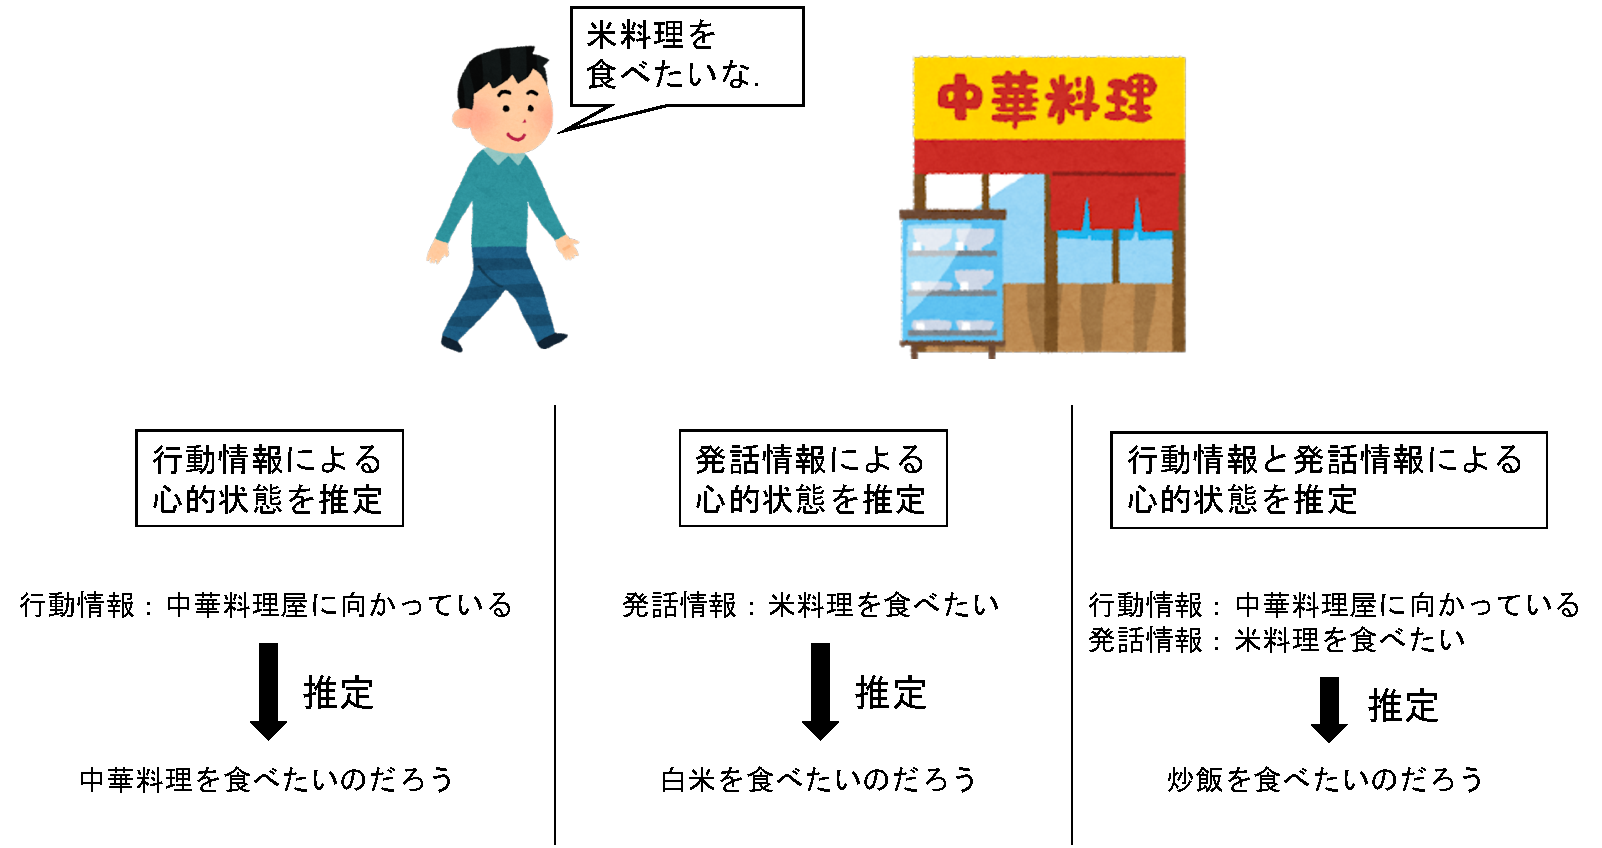
\includegraphics[scale=0.58]{./figure1.pdf}
    \caption{心的状態の推定.人間が食事をとるために飲食店に向かう場面において,3通りの条件で心的状態を推定する.図の左側は,行動情報のみを活用して心的状態を推定した場合,図の中央は発話情報のみを活用して心的状態を推定した場合,図の右側は行動情報と発話情報の両方を活用して心的状態を推定した場合を表す.}
    \label{fig:fig1}
  \end{center}
\end{figure}
人間は,気分が落ち込んでいる対話相手の発話に対してネガティブな発話解釈をしたり,励ましの言葉をかけるように,対話相手の心的状態によって相手の発話の解釈を変えたり,自身の発話の内容を変えている.また,相手が知らないことについて詳しく説明したり,相手が好むことについて話を掘り下げる.対話システムにおいても,人間と同様に対話相手の心的状態に合わせて,発話解釈を変えたり,自身の発話の内容を変えることで,より自然でありストレスの少ない対話を実現することができる.つまり,対話相手に合わせた臨機応変な発話解釈や発話生成により対話における不自然さやストレスをなくすためには,対話相手の心的状態を推定することが必要となる.


\par
人間の心的状態を推定する研究には,人間の行動情報から心的状態を推定する研究と発話情報から心的状態を推定する研究が存在する.人間の行動情報から心的状態を推定する研究は,代表的には,環境の状態と環境中を移動する人間の行動や観測状況,信念をベイズ推論に適用し,環境中を移動する人間の信念と欲求を推定する研究 \cite{baker2011bayesian}があげられる.発話情報から心的状態を推定する研究では,代表的には,発話から得られた事象を信念と捉え,考えられる欲求の候補を生成し,尤もらしい欲求を基に発話者の意図を推定する研究 \cite{高橋拓誠2015bdi}があげられる.また,心的状態を考慮することによる検索精度の向上のために,検索クエリへの入力から人間の心的状態を推定する研究 \cite{10.1007/978-3-642-02481-8_4}も存在する.

\par
従来研究では,行動情報のみから人間の心的状態を推定する研究や発話情報のみから人間の心的状態を推定する研究は存在した.しかし,行動情報と発話情報の両方を活用し人間の心的状態を推定する研究はない.従来研究における心的状態の推定は,遠くから行動を観測している場合や立ち止まって対話をしている場合というように,行動情報のみが観測される場合や発話情報のみが観測される場合には有効である.しかし実世界では,歩きながら対話を行う場合のように,行動情報と発話情報の両方が観測されることが多く,発話情報によって行動情報の解釈が変わったり,行動情報によって発話情報が変わることがある.例えば,外出への準備において忙しく行動している人を観測した時,「急いでいるのだろう」という解釈をする.しかし「出発まで,たくさん時間があります」という発話を受けた時,「行動力がある人だ」という解釈に変わる.また,上司から「なんでも聞いてください」という発話を受けた時,上司が忙しく行動してれば「今は聞くべきではない」と解釈することもある.従来研究では,行動情報と発話情報の両方が観測される場合においては,発話情報による行動情報の解釈の変化や,行動情報による発話情報の解釈の変化を捉えることが難しい.つまり,行動と発話の両方が観測される場合における従来研究における心的状態の推定では,行動と発話の相互作用の考慮による推定性能の向上の可能性が低いことが予想される.

\par
本研究では,行動情報と発話情報の両方から人間の心的状態を推定するシステムMultimodal Inference of Mind SCAIN (MIoM SCAIN)を提案する.MIoM SCAINは,行動情報と発話情報の両方を活用しベイズ推論によって人間の心的状態の一部である信念および欲求を推定する.MIoM SCAINは,人間の信念および欲求の推定において,信念と欲求の組み合わせをを一つに決め付けるのではなく,同時に複数保持し,やり取りの中でその可能性を動的に変えていく.MIoM SCAINは,行動情報と発話情報をもとに,複数保持した信念と欲求の組み合わせの可能性が大きく変動したタイミングまたは一定の時間,変動割合が小さかったタイミングで人間に質問を提示し,質問の応答を発話情報として推定に反映することで,発話情報による行動情報の解釈の変化や行動情報による発話情報の解釈の変化を捉え,行動情報と発話情報の相互作用を考慮した推定が可能となる.実験では,独自で作成したデータセットを利用し,MIoM SCAINにより信念と欲求の推定を行い,行動情報と発話情報の両方を推定に活用することが有効であるかを評価する.

\par
本論文の構成は以下の通りである.第二章では,関連研究においてどのように人間の心的状態を推定していたかを述べる.第三章では,人間の行動情報と発話情報から心的状態を推定するシステムMIoM SCAINを提案する.第四章では,MIoM SCAINと単一の情報のみから心的状態を推定するシステムを用いて実験的に評価し,第五章では評価結果について考察する.第六章では,MIoM SCAINにおける今後の課題について述べる.最後に,第七章で本論文を締めくくる.
